\begin{figure}
    \centering
    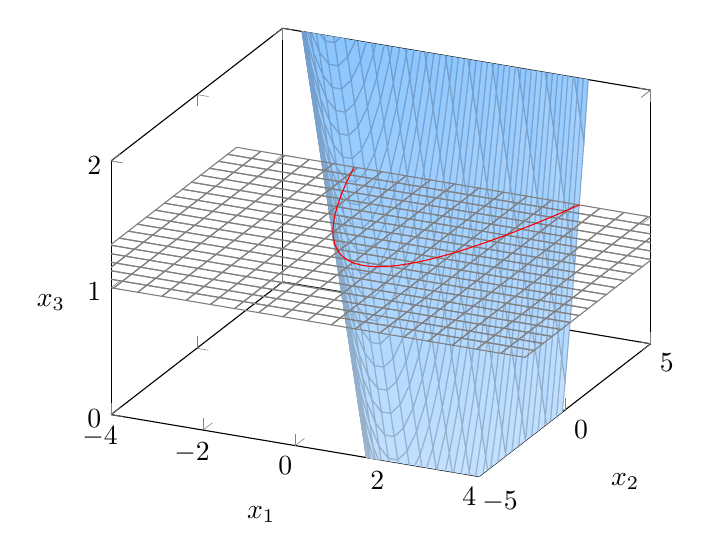
\begin{tikzpicture}
        \begin{axis}
            [
            xlabel=$x_1$,
            ylabel=$x_2$,
            zlabel=$x_3$,
            zlabel style={rotate = -90},
            xmin=-4, xmax=4,
            ymin=-5, ymax=5,
            zmin=0, zmax=2,
            ]
            \addplot3[surf, shader=faceted,samples=50,colormap/cool]{x*x-y};
            \addplot3[mesh,samples=20,color=gray](x,y,1);
            \addplot3[samples y=0,domain=-sqrt(6):sqrt(6),color=red]({x},{x*x - 1},{1});
        \end{axis}
    \end{tikzpicture}
    \caption{Caption}
    \label{fig:enter-label}
\end{figure}

\begin{figure}
    \centering
    \begin{tikzpicture}
        \begin{axis}
            [
            xlabel=$x_1$,
            ylabel=$x_2$,
            zlabel=$x_3$,
            zlabel style={rotate = -90},
            xmin=-4, xmax=4,
            ymin=-5, ymax=5,
            zmin=0, zmax=2,
            ]
            \addplot3[surf,shader=interp,samples=50,variable=\u, variable y=\v,domain=-sqrt(6):sqrt(6),y domain=0:1,colormap name=below]({u},{u*u - v},{v});
            \addplot3[mesh,samples=20,color=gray](x,y,1);
            \addplot3[mesh,samples=20,variable=\u, variable y=\v,domain=-sqrt(6):sqrt(6),y domain=1:2,colormap name=above]({u},{u*u - v},{v});
        \end{axis}  
    \end{tikzpicture}
    \caption{Caption}
    \label{fig:enter-label}
\end{figure}

\begin{figure}
    %\centering
    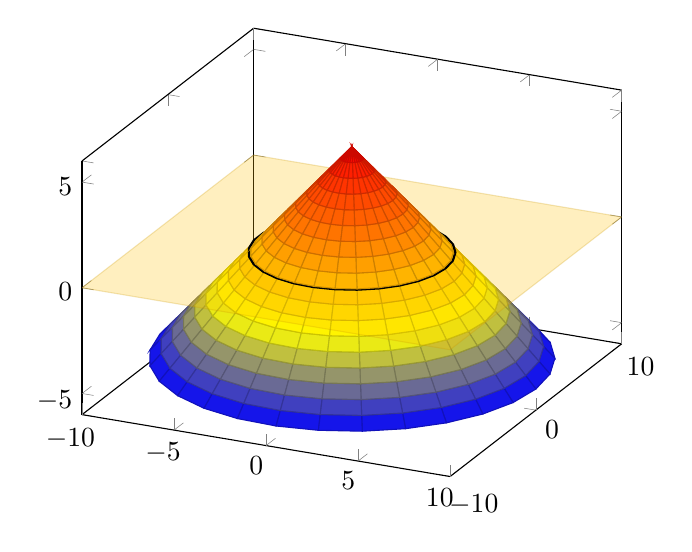
\begin{tikzpicture}
        \begin{axis}
            [
           z buffer=sort,data cs=polar 
            ]
            \addplot3[surf,domain=0:360,domain y=5:10, samples=30,samples y =10]{-y+5};
            \addplot3 [data cs=cart,surf,domain=-10:10, samples=2,opacity=0.25]{0};
            \addplot3[domain=0:360,samples y=0,samples=30,thick,z buffer=auto]({x},{5.1},{0});
            \addplot3[surf,domain=0:360, domain y=0:5,samples=30,samples y=10 ]{-y+5};
        \end{axis}
    \end{tikzpicture}
    \caption{Caption}
    \label{fig:enter-label}
\end{figure}

\begin{figure}
    \centering
    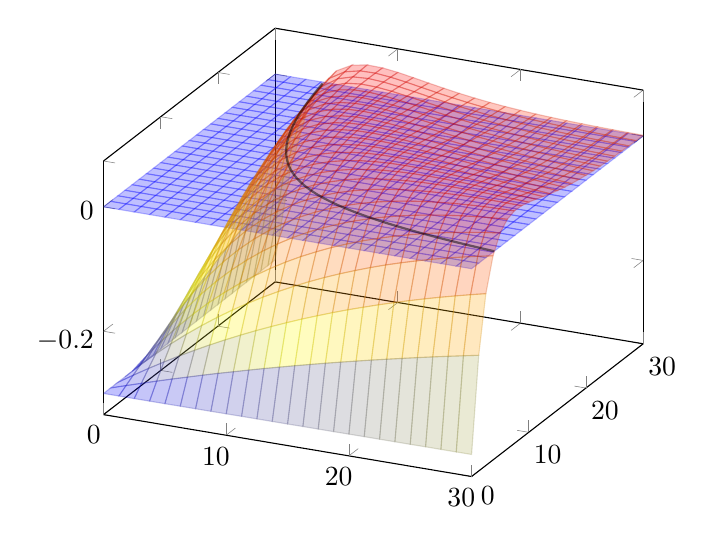
\begin{tikzpicture}
    \begin{axis}[domain=0.01:30]
    \addplot3[surf, opacity=0.25, blue, shader=flat] {0};
    \addplot3[surf, opacity=0.25] {(1-0.3)*e^(-x*(y/100)*(1-0.3))-e^(-x*(y/100))};
    \addplot3+[domain=4:30,samples=80,samples y=0,mark=none,black, opacity=0.5,thick]({x},{118.89/x},{0.});
\end{axis}
\end{tikzpicture}
    \caption{Caption}
    \label{fig:enter-label}
\end{figure}